%% ---------------------------------------------------------------------
\section{Results, limitations and future improvements}
\label{sec:discussion}

\subsection{Summary of results}

\begin{itemize}[leftmargin=*,itemsep=1pt]
  \item \textbf{Real vehicle.} Nav2 flew an autonomous square path around trees,
    outdoors at night, and a \SI{7}{\minute} GNSS-free \code{GUIDED} hover at \SI{2.5}{\metre} over grass drifted
    \SI{1.6}{\metre} (\cref{sec:val-hwdemo}).
  \item \textbf{Simulation} (26 flights, \SI{1.7}{h}, Gazebo truth). Three complete
    office explorations (about \SI{100}{m} and 7--8 minutes each, two without contact);
    speed limits held (95th percentile $\le$\SI{0.52}{m/s}); height RMS 3--\SI{14}{cm}.
    Four falls exposed height sag when braking and too small a margin to the propellers
    (\cref{tab:simincidents}).
  \item \textbf{System.} LiDAR, flow odometry, Nav2, semantic perception and health
    monitoring added to an unmodified ArduPilot multirotor with USB-only connections;
    a five-layer safety-gated command path with pilot override.
  \item \textbf{Link.} Software-path latency reduced to single-digit milliseconds
    (\cref{tab:latency}), with fragmentation-free encodings and per-stream metrics.
  \item \textbf{Need for exteroception.} Inertial-only integration on real autopilot data
    drifted \SI{86.5}{\metre} in \SI{25}{\second} (\SI{4.6}{\metre} after bias removal);
    the ZUPT detector has an order-of-magnitude margin at rest.
  \item \textbf{Perception.} Hybrid YOLO--SAM runs at \SI{31.6}{\milli\second} per frame,
    twice the camera rate; 17/17 logic tests pass.
\end{itemize}

\subsection{Status against the KPIs}

\begin{table}[H]
\centering\small
\caption{Verification status of each KPI for the current prototype.}
\label{tab:kpistatus}
\begin{tabularx}{\textwidth}{p{2.8cm} p{3.2cm} L}
\toprule
\textbf{KPI} & \textbf{Status} & \textbf{Evidence / gap} \\
\midrule
Trajectory error $<0.5\%$ & Not measured & Requires flights with ground truth (motion capture, surveyed markers or total station). The trade study predicts 1.4--1.5\% for the prototype's sensing, i.e.\ above target \\
Hover drift $\le\pm$\SI{5}{\centi\metre}/\SI{10}{\minute} & Not met & \SI{1.6}{\metre} over \SI{7}{\minute} in flight (\cref{sec:val-hwdemo}); about 10$\times$ better than GNSS-free fallback, over 30$\times$ the target \\
State $\ge$\SI{100}{\hertz}, vision $\ge$\SI{30}{\hertz} & Partly & Ground \topic{/odom} $\approx$\SI{30}{\hertz} (autopilot EKF runs faster internally). Camera $\approx$\SI{15}{\hertz}, limited by the USB camera. Perception capacity 32\,FPS \\
Compute $\le$\SI{15}{\watt} onboard & Not met by design & Processing is off-board on a GPU laptop in the prototype \\
\SIrange{0}{10000}{lux} & Partly & LiDAR and flow-based navigation is illumination-independent by principle. Camera perception is not. Untested \\
Endurance $\ge$\SI{30}{\minute} & Not met & Target battery is recorded as $\approx$\SI{10}{\minute} \\
\bottomrule
\end{tabularx}
\end{table}

\begin{figure}[H]
\centering
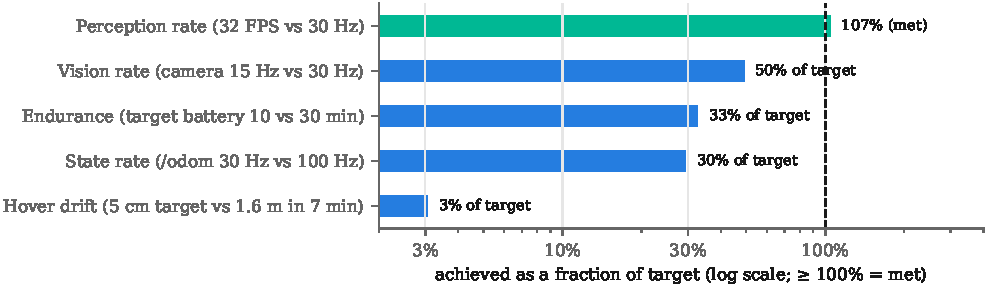
\includegraphics[width=0.85\textwidth]{kpi_status.pdf}
\caption{Measurable KPIs as a fraction of their targets (log scale). Trajectory error
(not yet measured), onboard compute (off-board by design) and illumination (untested)
are omitted. Hover drift is target over achieved, so 3\% means 32 times the
allowed drift.}
\label{fig:kpistatus}
\end{figure}

\subsection{Limitations}
\label{sec:limitations}

\begin{enumerate}[leftmargin=*,itemsep=2pt]
  \item \textbf{Limited flight validation on hardware.} This is the main gap. Our
    hover-drift figure (\SI{1.6}{\metre} in \SI{7}{\minute}) comes from a single run at
    \SI{2.5}{\metre} over grass, and the square-path flight had no external reference.
    We therefore cannot yet report trajectory error, avoidance success rate or
    over-the-air latency. The drift is also more than 30 times our KPI. We suspect the
    grass (its texture is low and repetitive, and it moves in the propeller downwash),
    the coarser flow resolution at \SI{2.5}{\metre}, and EKF tuning; repeating the test
    over a textured mat at \SIrange{1}{1.5}{\metre} should tell these apart. The
    simulation results (\cref{sec:val-simlogs}) use idealised sensors and cannot stand in
    for real flights.
  \item \textbf{Collision margin in simulation.} Four of nine simulated office flights
    contained a fall after propeller contact (\cref{tab:simincidents}). The bridge's
    \SI{0.65}{m} stop distance is measured from the LiDAR, while the propellers reach
    about \SI{0.38}{m} from the centre. Braking height dips of up to \SI{47}{cm} brought
    the vehicle down to the height of furniture the LiDAR cannot see. We need to fix both
    before flying the real vehicle indoors.
  \item \textbf{Off-board dependence.} Planning and perception require the Wi-Fi link.
    If the link drops, the
    stale-command stop and autopilot hold bring the vehicle to a safe halt, but the
    mission ends there. This is why the final design moves all processing onboard.
  \item \textbf{Odometry without loop closure.} On the real vehicle Nav2 runs in a
    rolling \code{odom} frame, and SLAM is used only in simulation. Flow-based
    dead-reckoning drifts with distance, and there is no covariance-weighted fusion of
    flow, LiDAR and IMU on the ground. The \code{/odom} covariance is not modelled.
  \item \textbf{2D sensing in a 3D world.} The LiDAR sees a single horizontal
    slice, so anything above or below it is invisible. We designed the simulated office
    around this limitation. The
    \code{scan_to_3d} map is built for inspection and does not feed the costmaps.
  \item \textbf{Placeholder extrinsics.} The LiDAR and camera mount transforms are
    estimates and must be calibrated for each build.
  \item \textbf{Optical-flow assumptions.} Conversion assumes a flat floor and correct
    \code{FLOW_ORIENT_YAW}. Flow quality falls over textureless or reflective floors,
    and samples below quality 20 are dropped, so velocity becomes zero.
  \item \textbf{Simulation--reality gap.} The simulation uses PX4 OFFBOARD with
    simulated GNSS in the estimator. The vehicle uses ArduPilot \code{GUIDED} without
    GNSS. The LiDAR safety filter exists only in the simulation bridge.
  \item \textbf{Screening estimates.} The trade-study figures are literature-typical
    values, not measurements.
\end{enumerate}

\subsection{Future improvements}

Ordered by our timeline (\cref{tab:timeline}) and by the gaps above:
\begin{enumerate}[leftmargin=*,itemsep=2pt]
  \item \textbf{Flight validation campaign.} Repeated hover-drift and figure-of-eight
    trajectory tests against an external reference. Report RMSE absolute trajectory
    error, drift as a percentage of distance, avoidance success rate, and the
    over-the-air latency distribution from \topic{/metrics/*/latency_ms}.
  \item \textbf{Fix the collision causes found in simulation.}
    \begin{itemize}[nosep]
      \item Measure the safety distances from the propeller envelope, not from the
        LiDAR.
      \item Hold height while braking.
      \item Add a regression test that replays the office exploration and fails on any
        fall (our log analysis already detects falls).
      \item Repeat the analysis with GPS disabled in EKF2, using SLAM or flow as the
        position source.
    \end{itemize}
  \item \textbf{Real-vehicle SLAM and fusion.} Run SLAM~Toolbox on the real scan stream
    to provide \code{map}$\rightarrow$\code{odom} and loop closure. Feed the resulting
    pose back to EKF3 as external navigation (MAVLink \code{VISION_POSITION_ESTIMATE}
    or \code{ODOMETRY}), so the autopilot's estimate is bounded and not only the
    planner's.
  \item \textbf{Port the LiDAR safety filter} from the simulation bridge to the Pi
    listener, so it acts even when the ground link is degraded.
  \item \textbf{Migrate onboard} to the design target. Use a Raspberry Pi~5 with stereo
    VIO (ORB-SLAM3 or VINS-Fusion), PX4 on the Kakute H7, and the existing link layer
    kept only for telemetry. Measure power against the \SI{15}{\watt} budget.
  \item \textbf{Perception on embedded hardware.} Measure YOLO-only and
    reduced-resolution SAM on the Pi~5 or an accelerator. Project segmentation masks
    into the costmap as a semantic layer.
  \item \textbf{Language-commanded navigation} (objective 11). A prototype
    (\code{scripts/context_learning.py}) already resolves object references against a
    JSON object list with an LLM. Integrate it with the semantic map, and validate
    every LLM-generated goal against the costmap before execution.
  \item \textbf{Degraded-condition tests}: darkness, smoke, glare, blocked camera, and
    saturated IMU (objectives 3 and 5).
  \item \textbf{Open-hardware completeness.} An archived release with DOI.
\end{enumerate}

\begin{table}[H]
\centering\small
\caption{Project timeline and status (\code{docs/TIMELINE.md}).}
\label{tab:timeline}
\begin{tabularx}{\textwidth}{l p{2.2cm} L}
\toprule
\textbf{Phase} & \textbf{Weeks} & \textbf{Scope (milestone)} \\
\midrule
0 Concept & done & Problem statement, 15-solution survey, scoring, design choice, BOM \\
1 Hardware & 1--3 & Procure target parts, PX4 on Kakute H7, test rig, ELRS and failsafes (manual flight) \\
2 Sensing & 3--6 & Stereo calibration, rectified images $\ge$\SI{30}{\hertz}, depth, IMU-only baseline \\
3 Estimation \& SLAM & 6--9 & VIO, EKF/factor-graph fusion, loop closure, KPI measurement (bounded drift) \\
4 Planning & 9--11 & Costmaps from depth, Nav2 tuning, static/dynamic avoidance \\
5 Language & 11--13 & LLM goal grounding with costmap validation (``go to the window'') \\
6 Full system & 13--16 & End-to-end GPS-free mission, degraded-condition tests, KPI sign-off \\
\bottomrule
\end{tabularx}
\end{table}

\noindent The prototype and simulation stack described here serve as our development
platform for phases 1--4. We expect the link, safety, planning and perception layers to
carry over to the onboard design largely unchanged.
